\documentclass{standalone}
\usepackage{tikz}
\usetikzlibrary{patterns, positioning}


\begin{document}
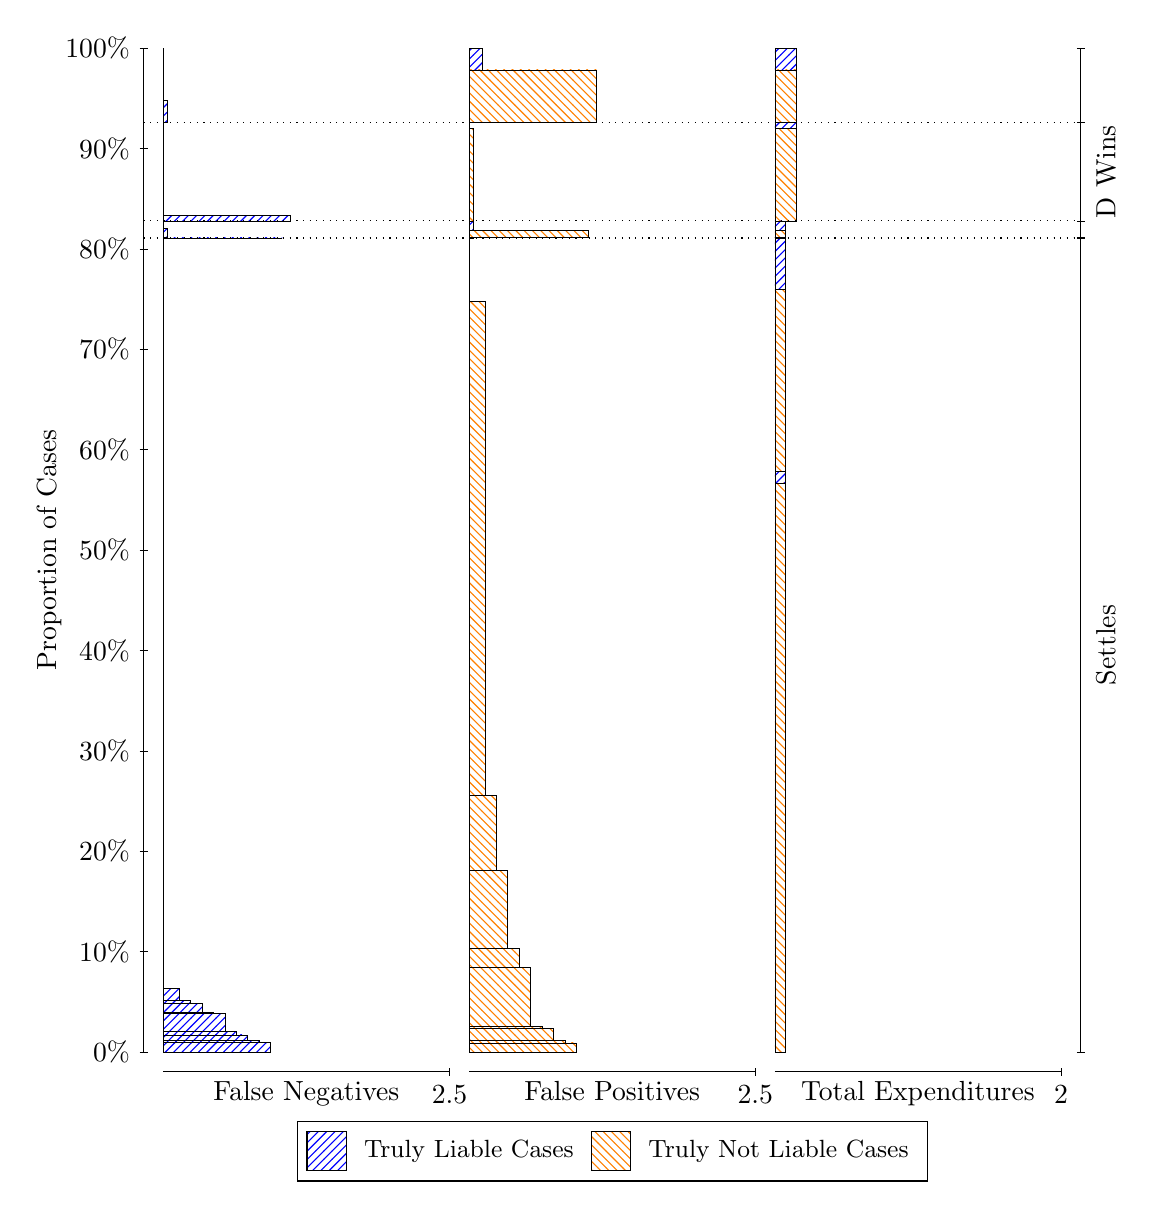
\begin{tikzpicture}
\draw[black, very thin] (1.5,1.75) -- (1.5,14.5);
\node[rotate=90, text=black, anchor=center] at (0.3, 8.125) {Proportion of Cases};
\draw[black, very thin] (1.45,1.75) -- (1.55,1.75);
\node[text=black, anchor=east] at (1.45, 1.75) {0\%};
\draw[black, very thin] (1.45,3.025) -- (1.55,3.025);
\node[text=black, anchor=east] at (1.45, 3.025) {10\%};
\draw[black, very thin] (1.45,4.3) -- (1.55,4.3);
\node[text=black, anchor=east] at (1.45, 4.3) {20\%};
\draw[black, very thin] (1.45,5.575) -- (1.55,5.575);
\node[text=black, anchor=east] at (1.45, 5.575) {30\%};
\draw[black, very thin] (1.45,6.85) -- (1.55,6.85);
\node[text=black, anchor=east] at (1.45, 6.85) {40\%};
\draw[black, very thin] (1.45,8.125) -- (1.55,8.125);
\node[text=black, anchor=east] at (1.45, 8.125) {50\%};
\draw[black, very thin] (1.45,9.4) -- (1.55,9.4);
\node[text=black, anchor=east] at (1.45, 9.4) {60\%};
\draw[black, very thin] (1.45,10.675) -- (1.55,10.675);
\node[text=black, anchor=east] at (1.45, 10.675) {70\%};
\draw[black, very thin] (1.45,11.95) -- (1.55,11.95);
\node[text=black, anchor=east] at (1.45, 11.95) {80\%};
\draw[black, very thin] (1.45,13.225) -- (1.55,13.225);
\node[text=black, anchor=east] at (1.45, 13.225) {90\%};
\draw[black, very thin] (1.45,14.5) -- (1.55,14.5);
\node[text=black, anchor=east] at (1.45, 14.5) {100\%};

\draw[black, very thin] (13.4,1.75) -- (13.4,14.5);
\draw[black, very thin] (13.35,1.75) -- (13.45,1.75);
\node[anchor=west] at (13.35, 1.75) {};
\draw[black, very thin] (13.35,12.088) -- (13.45,12.088);
\node[anchor=west] at (13.35, 12.088) {};
\draw[black, very thin] (13.35,12.094) -- (13.45,12.094);
\node[anchor=west] at (13.35, 12.094) {};
\draw[black, very thin] (13.35,12.305) -- (13.45,12.305);
\node[anchor=west] at (13.35, 12.305) {};
\draw[black, very thin] (13.35,13.553) -- (13.45,13.553);
\node[anchor=west] at (13.35, 13.553) {};
\draw[black, very thin] (13.35,14.5) -- (13.45,14.5);
\node[anchor=west] at (13.35, 14.5) {};

\draw[black, very thin, pattern color=blue, pattern=north east lines] (1.75,1.75) rectangle (3.1125,1.8696);
\draw[black, very thin, pattern color=blue, pattern=north east lines] (1.75,1.8696) rectangle (2.9672,1.8965);
\draw[black, very thin, pattern color=blue, pattern=north east lines] (1.75,1.8965) rectangle (2.8218,1.9684);
\draw[black, very thin, pattern color=blue, pattern=north east lines] (1.75,1.9684) rectangle (2.6765,2.0105);
\draw[black, very thin, pattern color=blue, pattern=north east lines] (1.75,2.0105) rectangle (2.5312,2.2422);
\draw[black, very thin, pattern color=blue, pattern=north east lines] (1.75,2.2422) rectangle (2.3858,2.257);
\draw[black, very thin, pattern color=blue, pattern=north east lines] (1.75,2.257) rectangle (2.2405,2.3717);
\draw[black, very thin, pattern color=blue, pattern=north east lines] (1.75,2.3717) rectangle (2.0952,2.4059);
\draw[black, very thin, pattern color=blue, pattern=north east lines] (1.75,2.4059) rectangle (1.9498,2.5545);
\draw[black, very thin, pattern color=orange, pattern=north west lines] (1.75,2.5545) rectangle (1.75,12.088);
\draw[black, very thin, pattern color=blue, pattern=north east lines] (1.75,12.088) rectangle (3.2578,12.088);
\draw[black, very thin, pattern color=orange, pattern=north west lines] (1.75,12.088) rectangle (1.75,12.094);
\draw[black, very thin, pattern color=blue, pattern=north east lines] (1.75,12.094) rectangle (1.8045,12.213);
\draw[black, very thin, pattern color=orange, pattern=north west lines] (1.75,12.213) rectangle (1.75,12.305);
\draw[black, very thin, pattern color=blue, pattern=north east lines] (1.75,12.305) rectangle (3.3668,12.379);
\draw[black, very thin, pattern color=orange, pattern=north west lines] (1.75,12.379) rectangle (1.75,13.553);
\draw[black, very thin, pattern color=blue, pattern=north east lines] (1.75,13.553) rectangle (1.8045,13.831);
\draw[black, very thin, pattern color=orange, pattern=north west lines] (1.75,13.831) rectangle (1.75,14.5);
\draw[black, very thin, pattern color=orange, pattern=north west lines] (5.6333,1.75) rectangle (6.9958,1.8656);
\draw[black, very thin, pattern color=orange, pattern=north west lines] (5.6333,1.8656) rectangle (6.8505,1.8989);
\draw[black, very thin, pattern color=orange, pattern=north west lines] (5.6333,1.8989) rectangle (6.7052,2.049);
\draw[black, very thin, pattern color=orange, pattern=north west lines] (5.6333,2.049) rectangle (6.5598,2.0769);
\draw[black, very thin, pattern color=orange, pattern=north west lines] (5.6333,2.0769) rectangle (6.4145,2.8206);
\draw[black, very thin, pattern color=orange, pattern=north west lines] (5.6333,2.8206) rectangle (6.2692,3.0621);
\draw[black, very thin, pattern color=orange, pattern=north west lines] (5.6333,3.0621) rectangle (6.1238,4.0551);
\draw[black, very thin, pattern color=orange, pattern=north west lines] (5.6333,4.0551) rectangle (5.9785,5.0105);
\draw[black, very thin, pattern color=orange, pattern=north west lines] (5.6333,5.0105) rectangle (5.8332,11.283);
\draw[black, very thin, pattern color=blue, pattern=north east lines] (5.6333,11.283) rectangle (5.6333,12.088);
\draw[black, very thin, pattern color=orange, pattern=north west lines] (5.6333,12.088) rectangle (5.6878,12.094);
\draw[black, very thin, pattern color=blue, pattern=north east lines] (5.6333,12.094) rectangle (5.6333,12.094);
\draw[black, very thin, pattern color=orange, pattern=north west lines] (5.6333,12.094) rectangle (7.1412,12.186);
\draw[black, very thin, pattern color=blue, pattern=north east lines] (5.6333,12.186) rectangle (5.6878,12.305);
\draw[black, very thin, pattern color=orange, pattern=north west lines] (5.6333,12.305) rectangle (5.6878,13.479);
\draw[black, very thin, pattern color=blue, pattern=north east lines] (5.6333,13.479) rectangle (5.6333,13.553);
\draw[black, very thin, pattern color=orange, pattern=north west lines] (5.6333,13.553) rectangle (7.2502,14.222);
\draw[black, very thin, pattern color=blue, pattern=north east lines] (5.6333,14.222) rectangle (5.7968,14.5);
\draw[black, very thin, pattern color=orange, pattern=north west lines] (9.5167,1.75) rectangle (9.6529,8.978);
\draw[black, very thin, pattern color=blue, pattern=north east lines] (9.5167,8.978) rectangle (9.6529,9.1245);
\draw[black, very thin, pattern color=orange, pattern=north west lines] (9.5167,9.1245) rectangle (9.6529,11.43);
\draw[black, very thin, pattern color=blue, pattern=north east lines] (9.5167,11.43) rectangle (9.6529,12.088);
\draw[black, very thin, pattern color=orange, pattern=north west lines] (9.5167,12.088) rectangle (9.6529,12.094);
\draw[black, very thin, pattern color=blue, pattern=north east lines] (9.5167,12.094) rectangle (9.6529,12.094);
\draw[black, very thin, pattern color=orange, pattern=north west lines] (9.5167,12.094) rectangle (9.6529,12.186);
\draw[black, very thin, pattern color=blue, pattern=north east lines] (9.5167,12.186) rectangle (9.6529,12.305);
\draw[black, very thin, pattern color=orange, pattern=north west lines] (9.5167,12.305) rectangle (9.7892,13.479);
\draw[black, very thin, pattern color=blue, pattern=north east lines] (9.5167,13.479) rectangle (9.7892,13.553);
\draw[black, very thin, pattern color=orange, pattern=north west lines] (9.5167,13.553) rectangle (9.7892,14.222);
\draw[black, very thin, pattern color=blue, pattern=north east lines] (9.5167,14.222) rectangle (9.7892,14.5);
\draw[black, dotted] (1.5,12.088) -- (13.4,12.088);
\draw[black, dotted] (1.5,12.094) -- (13.4,12.094);
\draw[black, dotted] (1.5,12.305) -- (13.4,12.305);
\draw[black, dotted] (1.5,13.553) -- (13.4,13.553);
\draw[black, very thin] (1.75,1.5) -- (5.3833,1.5);
\node[text=black, anchor=north] at (3.5667, 1.5) {False Negatives};
\draw[black, very thin] (5.3833,1.45) -- (5.3833,1.55);
\node[text=black, anchor=north] at (5.3833, 1.45) {2.5};

\draw[black, very thin] (5.6333,1.5) -- (9.2667,1.5);
\node[text=black, anchor=north] at (7.45, 1.5) {False Positives};
\draw[black, very thin] (9.2667,1.45) -- (9.2667,1.55);
\node[text=black, anchor=north] at (9.2667, 1.45) {2.5};

\draw[black, very thin] (9.5167,1.5) -- (13.15,1.5);
\node[text=black, anchor=north] at (11.333, 1.5) {Total Expenditures};
\draw[black, very thin] (13.15,1.45) -- (13.15,1.55);
\node[text=black, anchor=north] at (13.15, 1.45) {2};

\node[text=black, centered, rotate=90] at (13.72, 6.9188) {Settles};


\node[text=black, centered, rotate=90] at (13.72, 12.929) {D Wins};


\draw (7.449999999999999,1.5) node[draw=none] (baseCoordinate) {};
\begin{scope}[align=center]
        \matrix[scale=0.5, draw=black, below=0.5cm of baseCoordinate, nodes={draw}, column sep=0.1cm]{
            \node[rectangle, draw, minimum width=0.5cm, minimum height=0.5cm, pattern color=blue, pattern=north east lines] {}; &
            \node[draw=none, font=\small, text=black] (B) {Truly Liable Cases}; &
            \node[rectangle, draw, minimum width=0.5cm, minimum height=0.5cm, pattern color=orange, pattern=north west lines] {}; &
            \node[draw=none, font=\small, text=black] (B) {Truly Not Liable Cases}; \\
            };
\end{scope}

\end{tikzpicture}
\end{document}